\documentclass[10pt]{article}
\usepackage[utf8]{inputenc}
\usepackage[T1]{fontenc}
\usepackage{amsmath}
\usepackage{amsfonts}
\usepackage{amssymb}
\usepackage[version=4]{mhchem}
\usepackage{stmaryrd}
\usepackage{bbold}
\usepackage{graphicx}

\title{Gibbs Sampler}

\begin{document}
The Gibbs sampler is a Markov Chain Monte Carlo (MCMC) method used for sampling from the joint distribution of multiple variables when the form of the joint target distribution $$
\pi(x)=\pi\left(x_1, x_2, \ldots, x_d\right) .
$$
is complex and direct sampling is difficult. It is particularly useful in the context of Bayesian statistics for estimating the posterior distributions of parameters. The Gibbs sampler achieves this by iteratively sampling from the conditional distributions of each variable, holding all other variables fixed. There are two main variants of the Gibbs sampler based on how the variables are selected for updating in each iteration: the Systematic Scan Gibbs Sampler and the Random Scan Gibbs Sampler.

\section{Systematic Scan Gibbs Sampler}

The Systematic Scan Gibbs Sampler follows a predetermined order for updating each variable. In each iteration, it cycles through the variables in a specific sequence, updating one variable at a time based on its conditional distribution given the current values of all other variables. This process is repeated for a large number of iterations to ensure convergence to the target distribution. The systematic scan approach ensures that every variable is updated in a consistent manner, which can be advantageous for convergence properties in certain settings.
\newline
We use the standard notation $x_{-i}=\left(x_1, \ldots, x_{i-1}, x_{i+1}, \ldots, x_d\right)$.
\newline
\textbf{Algorithm}. Systematic scan Gibbs sampler. Let $\left(X_1^{(1)}, \ldots, X_d^{(1)}\right)$ be the initial state then iterate for $t=2,3, \ldots$
1. Sample $X_1^{(t)} \sim \pi_{X_1 \mid X_{-1}}\left(\cdot \mid X_2^{(t-1)}, \ldots, X_d^{(t-1)}\right)$. \newline
j. Sample $X_j^{(t)} \sim \pi_{X_j \mid X_{-j}}\left(\cdot \mid X_1^{(t)}, \ldots, X_{j-1}^{(t)}, X_{j+1}^{(t-1)}, \ldots, X_d^{(t-1)}\right)$. \newline
d. Sample $X_d^{(t)} \sim \pi_{X_d \mid X_{-d}}\left(\cdot \mid X_1^{(t)}, \ldots, X_{d-1}^{(t)}\right)$.\newline
The conditional distributions used in the Gibbs sampler are often referred to as full conditionals. A popular alternative to the systematic scan Gibbs sampler is the random scan Gibbs sampler.

or more intuitively:
\begin{enumerate}
    \item Initialize all variables \(x_1, x_2, \ldots, x_n\) to some starting values.
    \item For each iteration:
   - Sequentially update each variable \(x_i\) based on its conditional distribution given the current values of all other variables, i.e., \(p(x_i | x_{-i})\), where \(x_{-i}\) denotes all variables except \(x_i\).
\end{enumerate}
1. 
2. For each iteration:
    Sequentially update each variable \(x_i\) based on its conditional distribution given the current values of all other variables, i.e., \(p(x_i | x_{-i})\), where \(x_{-i}\) denotes all variables except \(x_i\).
3. Repeat step 2 for a large number of iterations to allow the Markov chain to converge to the target distribution.

\section{Random Scan Gibbs Sampler}

The Random Scan Gibbs Sampler, on the other hand, selects a variable to update at random in each iteration, rather than following a systematic order. This means that some variables may be updated more frequently than others in the short term, but over many iterations, each variable should be updated approximately equally on average. The random selection can potentially lead to faster mixing of the Markov chain in some cases, as it avoids the potentially slow traversal of the variable space that can occur with systematic scanning.

\textbf{Algorithm. }Random scan Gibbs sampler. Let $\left(X_1^{(1)}, \ldots, X_d^{(1)}\right)$ be the initial state then iterate for $t=2,3, \ldots$
\newline
\begin{enumerate}
    \item Sample an index $J$ from a distribution on $\{1, \ldots, d\}$ (typically uniform).
    \item  Sample $X_J^{(t)} \sim \pi_{X_J \mid X_{-J}}\left(\cdot \mid X_1^{(t-1)}, \ldots, X_{J-1}^{(t-1)}, X_{J+1}^{(t-1)}, \ldots, X_d^{(t-1)}\right)$ and set $X_k^{(t)}:=X_k^{(t-1)}$ for $k \neq J$
\end{enumerate}

or more intuitively:
\begin{enumerate}
    \item Initialize all variables \(x_1, x_2, \ldots, x_n\) to some starting values.
    \item For each iteration:
    \begin{enumerate}
        \item Randomly select a variable \(x_i\) to update.
        \item Update the selected variable \(x_i\) based on its conditional distribution given the current values of all other variables, i.e., \(p(x_i | x_{-i})\).
    \end{enumerate}
    \item Repeat step 2 for a large number of iterations to allow the Markov chain to converge to the target distribution.
\end{enumerate}
Both the Systematic Scan Gibbs Sampler and the Random Scan Gibbs Sampler are widely used in statistical computing for their ability to handle high-dimensional and complex distributions. The choice between systematic and random scanning can depend on the specifics of the problem at hand, including the structure of the conditional distributions and the desired convergence properties.


\begin{figure}
    \centering
    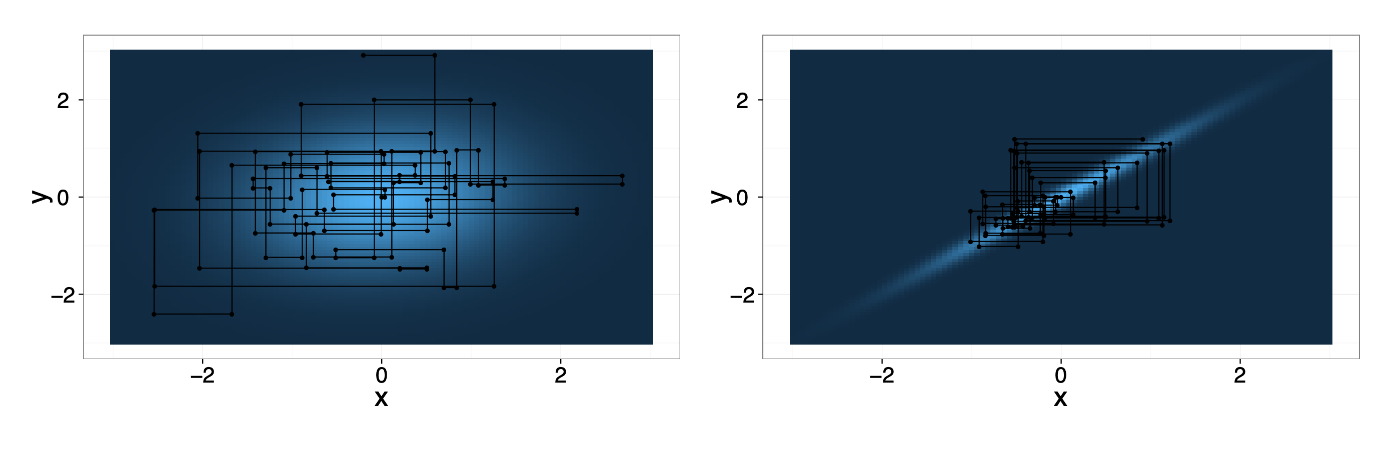
\includegraphics[width=1\linewidth]{overviews/MCMC/figures/slow-fast-mixing.png}
    \caption{Gibbs sampler on a bivariate normal distribution. Left: $\rho=0.1$, right $\rho=0.99$.}
    \label{fig:}
\end{figure}
\end{document}